\documentclass[tikz]{standalone}
\usepackage[x11names]{xcolor}
\usepackage[default,oldstyle]{sourcesanspro}

% See https://tex.stackexchange.com/a/445446 which was used as a template for
% this diagram below.
\usetikzlibrary{
  arrows.meta,
  calc,
  shapes.geometric,
  shapes.symbols,
  fit,
  positioning}
\tikzset{
  module/.style={%
    fill=white,
    draw=black, rounded corners,
    % Minimum height is useful to take into account capital
    % letters and such that take up extra height.
    minimum height=7mm,
    align=center,
    font=\sffamily
  },
  user/.style={%
    shape=ellipse,
    fill=white,
    draw=black, rounded corners,
    % Minimum height is useful to take into account capital
    % letters and such that take up extra height.
    minimum height=7mm,
    align=center,
    font=\sffamily
  },
  arrowX/.style={%
    {Latex[length=2mm,width=2mm]}-{Latex[length=2mm,width=2mm]}
  },
  arrowL/.style={%
    {Latex[length=2mm,width=2mm]}-
  },
  arrowR/.style={%
    -{Latex[length=2mm,width=2mm]}
  }%
}

\begin{document}
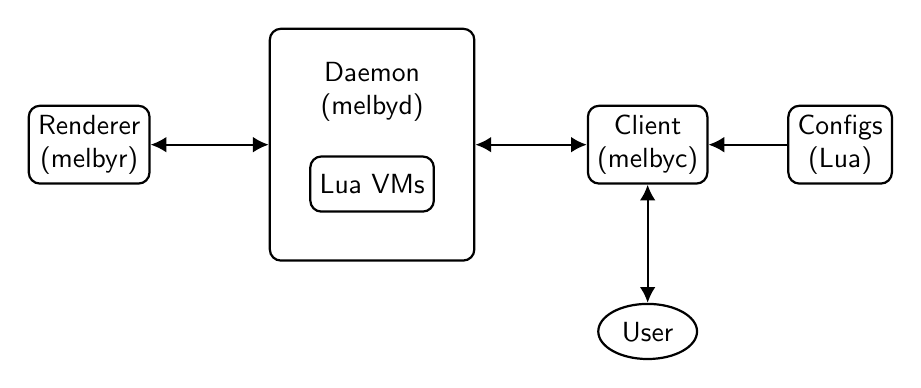
\begin{tikzpicture}[thick,font=\sffamily,every label/.append
    style={font=\sffamily,align=center}]

% Lua VMs. This is the "root" node as it does not reference anything
% else in terms of positioning.
\node[module, label={[yshift=3mm]Daemon\\(melbyd)}] (LuaVMs) {Lua VMs};
% Outer box around melbyd, which includes the LuaVMs.
\node[fit={(0,2) (LuaVMs) (0,-1)}, draw, rounded corners,
  inner xsep=5mm, inner ysep=-\pgflinewidth] (melbydOutline) {};
\node[module, left=1.5cm of melbydOutline] (melbyr) {Renderer\\(melbyr)};

% We could just use "right=1.5cm of melbydOutline" here but use calc's syntax
% for computing a coordinate combined with a (X,Y) delta for future reference in
% case we need to fine-tune an illustration.
\node[module] at ($(melbydOutline) + (3.5cm,0cm)$) (melbyc) {Client\\(melbyc)};
\node[module, right=1cm of melbyc] (Configs) {Configs\\(Lua)};
\node[user, below=1.5cm of melbyc] (User) {User};

\draw[arrowX] (melbyr)--(melbydOutline);
\draw[arrowX] (User)--(melbyc);
\draw[arrowL] (melbyc)--(Configs);
\draw[arrowX] (melbyc)--(melbydOutline);

\end{tikzpicture}
\end{document}
